\appendix
\chapter*{Appendices}
\addcontentsline{toc}{chapter}{Appendices}
\renewcommand{\thesection}{\Alph{section}}
\renewcommand{\theequation}{\thesection.\arabic{equation}}
\renewcommand{\thefigure}{H.\arabic{figure}} \quad \setcounter{figure}{0} % not very clean but it will do



\section{Cicalese and Vaccaro's original proof of supermodularity} \label{app:supermodularity}

This section goes over the original proof of Theorem \ref{th:shannon_supermodularity} for the Shannon entropy, taken from Ref. \cite{cicalese_supermodularity_2002}. The proof is mainly here for reader convenience, as the original paper is not easily accessible. The proof is structured in two lemmas. Note that the convention $0 \log \frac{1}{0} = 0$ is used (an event that never happens does not contribute to entropy). We will first need the following definition.

\begin{appendix_definition}[Inversion point]
    Let $p, q \in \mathcal{P}^d$. We say that the index $i \in \{2, \ldots, n\}$ is an \textit{inversion point} for $p$ and $q$ if either
\begin{equation}
    \sum_{l=1}^{i} p_l < \sum_{l=1}^{i} q_l \quad \text{and} \quad \sum_{l=1}^{i-1} p_l > \sum_{l=1}^{i-1} q_l    
\end{equation}
or, vice versa, if
\begin{equation}
    \sum_{l=1}^{i} p_l > \sum_{l=1}^{i} q_l \quad \text{and} \quad \sum_{l=1}^{i-1} p_l < \sum_{l=1}^{i-1} q_l.
\end{equation}
\end{appendix_definition}

\noindent Let $2 \leq i_1 < i_2 < \cdots < i_k \leq n$ be all and the only inversion points for $p, q \in \mathcal{P}^d$, and let
\begin{equation}
    t = (t_1, \ldots, t_n) = p \wedge q
\end{equation}
and
\begin{equation}
    s = (s_1, \ldots, s_n) = \beta(p, q).
\end{equation}

The first lemma is the following, where we assume $i_0 = 0$ and $i_{k+1} = n + 1$ for the sake of definiteness.

\begin{appendix_lemma} \label{lem:shannon_1}
    For each inversion point $i_r$, $r = 0, \ldots, k$, we have
    \begin{equation}
        \sum_{l=i_r+1}^{i_{r+1}-1} p_l \log \frac{1}{p_l} + q_l \log \frac{1}{q_l} = \sum_{l=i_r+1}^{i_{r+1}-1} t_l \log \frac{1}{t_l}.
    \end{equation}
\end{appendix_lemma} 

\begin{proof} Let us assume, without loss of generality, that
    \begin{equation}
        \sum_{l=1}^{i_r} p_l > \sum_{l=1}^{i_r} q_l.
    \end{equation}
    Then
    \begin{equation}
        \sum_{l=1}^{i_r} s_l = \sum_{l=1}^{i_r} p_l,
    \end{equation}
    and for all $s = i_r + 1, \ldots, i_{r+1} - 1$, we also have
    \begin{equation}
        s_s = \sum_{l=1}^{s} p_l - \sum_{l=1}^{s} q_l = p_s.
    \end{equation}
    Accordingly, we have
    \begin{equation}
        \sum_{l=1}^{i_r} t_l = \sum_{l=1}^{i_r} q_l,
    \end{equation}
    and for all $s = i_r + 1, \ldots, i_{r+1} - 1$, we have
    \begin{equation}
        t_s = \sum_{l=0}^{s} q_l - \sum_{l=0}^{s} t_l = q_s. \qedhere
    \end{equation}
\end{proof}

As an immediate consequence of Lemma \ref{lem:shannon_1}, we have
\begin{equation}
    \sum_{l=i_r+1}^{i_{r+1}-1} \left( p_l \log \frac{1}{p_l} + q_l \log \frac{1}{q_l} - t_l \log \frac{1}{t_l} \right) = 0.
\end{equation}

\begin{appendix_lemma} \label{lem:shannon_2}
    For each inversion point $i_r$, $r = 1, 2, \ldots, k$, we have
    \begin{equation}
        s_{i_r} \log \frac{1}{s_{i_r}} + t_{i_r} \log \frac{1}{t_{i_r}} > p_{i_r} \log \frac{1}{p_{i_r}} + q_{i_r} \log \frac{1}{q_{i_r}},
    \end{equation}
    where $p_{i_r}, q_{i_r}, s_{i_r}, t_{i_r} > 0$.
\end{appendix_lemma}

\begin{proof}
    Let us write $p, q, s, t$ instead of $p_{i_r}, q_{i_r}, s_{i_r}, t_{i_r}$, respectively. Without loss of generality let us assume that for the inversion point $i_r$ it holds that
    \begin{equation}
        \sum_{l=1}^{i_r} p_l > \sum_{l=1}^{i_r} q_l \quad \text{and} \quad \sum_{l=1}^{i_r-1} p_l < \sum_{l=1}^{i_r-1} q_l.
    \end{equation}
    It follows that $s > p$ and $q > t$, so $s > t$. Moreover, it is not hard to see that $s + t = p + q$. Let $s = q + \Delta$, then $t = p - \Delta$ and $s + t = p + q$. Then we have
    \begin{align}
        s \log \frac{1}{s} + t \log \frac{1}{t} - p \log \frac{1}{p} - q \log \frac{1}{q}
        &= - (s \log s + t \log t) + p \log p + q \log q \\
        &= - (q + \Delta) \log (q + \Delta) - (p - \Delta) \log (p - \Delta)\nonumber\\
        &\quad + p \log p + q \log q \\
        &= (q \log q + p \log p) - \left( (q + \Delta) \log (q + \Delta) \right.\nonumber\\
        &\quad \left. + (p - \Delta) \log (p - \Delta) \right) \\
        &\overset{\text{Jensen}}{\geq} (q + p + \Delta) \log \left( \frac{(q + p + \Delta)^2}{(q + \Delta)(p - \Delta)} \right) \label{eq:jensen_step} \\
        &= (q + p + \Delta) \log \left( \frac{s + t + \Delta}{s + \Delta} \cdot \frac{s + t + \Delta}{t - \Delta} \right) \\
        &= (q + p + \Delta) \log \left( \frac{(s + t + \Delta)^2}{(s + \Delta)(t - \Delta)} \right) > 0,
    \end{align}
    since $s > t$ and $\Delta < t$. The remaining case $s \leq t$ is completely symmetric, provided that we set $s = p + \Delta$ and $t = q - \Delta$. \qedhere
\end{proof}

Note that Eq. (\ref{eq:jensen_step}) invokes Jensen's inequality. We have not gone over it in this master thesis, but it is sufficient to know that in the discrete case it is essentially a (less general) form of Karamata's inequality (Lemma \ref{lem:karamata}). We are now ready to prove Theorem \ref{th:shannon_supermodularity}.

\begin{proof}[Proof of Theorem \ref{th:shannon_supermodularity}]
    We have
    \begin{align}
        H(s) + H(t) - H(p) - H(q)
        &= \sum_{l=1}^{k} \left( s_l \log \frac{1}{s_l} + t_l \log \frac{1}{t_l} - p_l \log \frac{1}{p_l} - q_l \log \frac{1}{q_l} \right) \\
        &= \sum_{r=1}^{k} \left( \sum_{l=i_r+1}^{i_{r+1}-1} \left( s_l \log \frac{1}{s_l} + t_l \log \frac{1}{t_l} \right)
        + s_{i_r} \log \frac{1}{s_{i_r}} + t_{i_r} \log \frac{1}{t_{i_r}} \right. \nonumber\\
        &\quad \left. - p_{i_r} \log \frac{1}{p_{i_r}} - q_{i_r} \log \frac{1}{q_{i_r}} 
        - \sum_{l=i_r+1}^{i_{r+1}-1} \left( p_l \log \frac{1}{p_l} + q_l \log \frac{1}{q_l} \right) \right) \nonumber \\
        &\quad + \sum_{l=1}^{i_1 - 1} \left( s_l \log \frac{1}{s_l} + t_l \log \frac{1}{t_l} 
        - p_l \log \frac{1}{p_l} - q_l \log \frac{1}{q_l} \right) \nonumber \\
        &\quad + \sum_{l=i_k+1}^{n} \left( s_l \log \frac{1}{s_l} + t_l \log \frac{1}{t_l} 
        - p_l \log \frac{1}{p_l} - q_l \log \frac{1}{q_l} \right) \\
        &\overset{\text{Lemma \ref{lem:shannon_1}}}{=} \sum_{r=1}^{k} \left( s_{i_r} \log \frac{1}{s_{i_r}} + t_{i_r} \log \frac{1}{t_{i_r}} 
        - p_{i_r} \log \frac{1}{p_{i_r}} \right.\nonumber\\
        &\quad \quad \quad \quad \quad \quad \quad \left.- q_{i_r} \log \frac{1}{q_{i_r}} \right) \\
        &\overset{\text{Lemma \ref{lem:shannon_2}}}{>} 0. \qedhere
    \end{align}
\end{proof}




\newpage

\section{Entropy of compositions of random variables} \label{app:shannon_compositions}

\setcounter{equation}{0}

This section is based on Ref. \cite[pp. 16--22]{cover_elements_2006}. In practice, we are often concerned with more than one process at a given time, and so defining the uncertainty of two variables $X$, $Y$ is interesting. Moreover, knowing how much measuring one variable reduces the uncertainty on the second one (and so how much information on the second process we gain) on average is valuable as well. These concepts are captured by \textit{joint entropy}, \textit{conditional entropy} and \textit{mutual information}.

\begin{appendix_definition}[Joint entropy]
    Let $X$ and $Y$ be random variables over alphabets $\mathcal{X}$ and $\mathcal{Y}$ with joint probability distribution $p(x, y)$. Then the joint entropy $H(X, Y)$ of $X$ and $Y$ is defined as
    \begin{align}
        H(X, Y) &= - \sum_{x \in \mathcal{X}, y \in \mathcal{Y}} p(x, y) \log p(x, y)\\
                &= - E[\log p(x, y)].
    \end{align}
\end{appendix_definition}

\begin{appendix_definition}[Conditional entropy]
    Let $X$ and $Y$ be random variables over alphabets $\mathcal{X}$ and $\mathcal{Y}$ with marginal probability distributions $p(x)$ and $p(y)$. Then the conditional entropy $H(X|Y)$ of $X$ knowing $Y$ is defined as
    \begin{align}
        H(X|Y) &= \sum_{y \in \mathcal{Y}} p(y) H(X|Y = y)\\
                 &= - \sum_{y \in \mathcal{Y}} p(y) \sum_{x \in \mathcal{X}} p(x|y) \log p(x|y)\\
                 &= - \sum_{y \in \mathcal{Y}} \sum_{x \in \mathcal{X}} p(x, y) \log p(x|y)\\
                 &= - E[\log p(x|y)].
    \end{align}
\end{appendix_definition}

It is interesting to note that these definitions are all very consistent with each other, as the vision of entropy being the expected value of the random variable $\log \frac{1}{p(x)}$ holds even for compositions of random variables. Before defining mutual information, we introduce another mathematical tool, the Kullback-Leibler divergence $D(p \parallel q)$ of two probability mass functions $p$ and $q$, sometimes called \textit{relative entropy}.

\begin{appendix_definition}[Kullback-Leibler divergence]
    Let $p$ and $q$ be two probability mass functions over an alphabet $\mathcal{X}$. Then the Kullback-Leibler divergence $D(p \parallel q)$ of $p$ and $q$ is defined as
    \begin{align}
        D(p \parallel q) &= \sum_{x \in \mathcal{X}} p(x) \frac{p(x)}{q(x)}\\
                &= E_p\left[\log \frac{p(x)}{q(x)}\right],
    \end{align}
    with conventions $0 \log \frac{0}{0} = 0$, $p \log \frac{p}{0} = \infty$ and $0 \log \frac{0}{q} = 0$ by continuity arguments.
\end{appendix_definition}

This quantity can be understood as measuring how far from each other the two distributions $p$ and $q$ are. If they are identical, i.e. $p(x) = q(x) \: \forall x \in \mathcal{X}$, then all of the terms in the sum are $\log \frac{p(x)}{p(x)} = \log 1 = 0$ and the relative entropy is simply 0. It is important to note however that this quantity is not a proper notion of distance, as it is not symmetric in its arguments, and fails the triangular inequality. % fort similaire a Cover and Thomas, faudrait reformuler un peu
Nonetheless, this notion of distance is used to define mutual information between two random variables as the Kullback-Leibler divergence between the joint probability distribution and the product of the marginal probability distributions.

\begin{appendix_definition}[Mutual information]
    Let $X$ and $Y$ be random variables over alphabets $\mathcal{X}$ and $\mathcal{Y}$ with marginal probability distributions $p(x)$ and $p(y)$ and joint distribution $p(x, y)$. Then the mutual information $I(X, Y)$ of $X$ and $Y$ is defined as
    \begin{align}
        I(X, Y) &= D(p(x, y)||p(x)p(y))\\
                &= \sum_{x \in \mathcal{X}} \sum_{y \in \mathcal{Y}} p(x, y) \log \frac{p(x, y)}{p(x)p(y)}\\
                &= E_{p(x, y)}\left[\log \frac{p(x, y)}{p(x)p(y)}\right]\\
                &= E_{p(x, y)}[- \log p(x)] + E_{p(x, y)}[- \log p(y)] - E_{p(x, y)}[- \log p(x, y)]\\
                &= E_{p(x)}[- \log p(x)] + E_{p(y)}[- \log p(y)] - E_{p(x, y)}[- \log p(x, y)]\\
                &= H(X) + H(Y) - H(X, Y).
    \end{align}
\end{appendix_definition}

Again, this definition agrees with what we would expect intuitively from a notion of the information that two random variables contain about each other: if the variables are independent, and thus contain no information about each other whatsoever (as the outcome of one does not affect the other), then their joint distribution reduces to the product of the marginal distributions, and the relative entropy in the definition becomes 0. Then, the less independent the joint distribution becomes, the farther it becomes from the product distribution, and the more measuring the outcome of one variable can tell you about the outcome of the second. It is interesting to note that the mutual information is symmetric in its arguments.

To finish this small incursion into classical information theory, it turns out that the Shannon entropy is actually the only function that satisfies all the properties that one would expect from a measure of information, such as (non-exhaustive list):

\begin{itemize}
    \item $H(X) \geq 0$.
    \item $H(X, Y) = H(Y, X)$.
    \item $H(X, Y) = H(X) + H(Y|X)$.
    \item \textbf{Subadditivity}\footnote{This subadditivity is not related to the subadditivity on the lattice.}\textbf{:} $H(X, Y) \leq H(X) + H(Y)$ with equality iff $X$ and $Y$ are independent.
    \item $H(X|Y) \leq H(X)$, which directly implies that $I(X, Y) \geq 0$, with equality iff $X$ and $Y$ are independent.
\end{itemize}



\newpage

\section{Mixed state example}
\label{app:mixed_example}

\setcounter{equation}{0}

Let us take a qubit, and let us try to find the difference between the states $\rho$ and $\rho'$ from the coin-flip example in Section \ref{sec:density_matrices}. In the computational basis, they are written
\begin{align}
    \rho &= 1/2 \ket{0}\bra{0} + 1/2 \ket{1}\bra{1} = \left(\begin{matrix}
        1/2 & 0\\
        0 & 1/2
    \end{matrix}\right),\\
    \rho' &= \ket{\psi}\bra{\psi} = \ket{+}\bra{+} = \frac{1}{\sqrt{2}}(\ket{0} + \ket{1})\frac{1}{\sqrt{2}}(\bra{0} + \bra{1}) = \left(\begin{matrix}
        1/2 & 1/2\\
        1/2 & 1/2
    \end{matrix}\right).
\end{align}

In both cases, let us measure if the qubit is in state $\ket{0}$ or $\ket{1}$. Those measurements are described by the operators $M_0 = \ket{0}\bra{0}$ and $M_1 = \ket{1}\bra{1}$, which are simple projective measurements. For $\rho$, we have
\begin{align}
    p(0) &= \tr\Big(\ket{0}\bra{0}\ket{0}\bra{0}\big(1/2 \ket{0}\bra{0} + 1/2 \ket{1}\bra{1}\big)\Big)\\
         &= \tr\Big(1/2 \ket{0}\bra{0}\ket{0}\bra{0} + 1/2 \ket{0}\bra{0}\ket{1}\bra{1}\Big)\\
         &= \tr(1/2 \ket{0}\bra{0}\ket{0}\bra{0})\\
         &= 1/2,
\end{align}
\begin{align}
    p(1) &= \tr\Big(\ket{1}\bra{1}\ket{1}\bra{1}\big(1/2 \ket{0}\bra{0} + 1/2 \ket{1}\bra{1}\big)\Big)\\
         &= \tr\Big(1/2 \ket{1}\bra{1}\ket{0}\bra{0} + 1/2 \ket{1}\bra{1}\ket{1}\bra{1}\Big)\\
         &= \tr(1/2 \ket{1}\bra{1}\ket{1}\bra{1})\\
         &= 1/2.
\end{align}
\noindent For $\rho'$, we have
\begin{align}
    p(0) &= \tr\Big(\ket{0}\bra{0}\ket{0}\bra{0}\big(1/2 \ket{0}\bra{0} + 1/2 \ket{0}\bra{1} + 1/2 \ket{1}\bra{0} 1/2 \ket{1}\bra{1}\big)\Big)\\
         &= \tr\Big(1/2 \ket{0}\bra{0}\ket{0}\bra{0} +1/2 \ket{0}\bra{0}\ket{0}\bra{1} + 1/2 \ket{0}\bra{0}\ket{1}\bra{0} + 1/2 \ket{0}\bra{0}\ket{1}\bra{1}\Big)\\
         &= \tr(1/2 \ket{0}\bra{0} + 1/2 \ket{0}\bra{1})\\
         &= 1/2,
\end{align}
\begin{align}
    p(1) &= \tr\Big(\ket{1}\bra{1}\ket{1}\bra{1}\big(1/2 \ket{0}\bra{0} + 1/2 \ket{0}\bra{1} + 1/2 \ket{1}\bra{0} 1/2 \ket{1}\bra{1}\big)\Big)\\
         &= \tr\Big(1/2 \ket{1}\bra{1}\ket{0}\bra{0} +1/2 \ket{1}\bra{1}\ket{0}\bra{1} + 1/2 \ket{1}\bra{1}\ket{1}\bra{0} + 1/2 \ket{1}\bra{1}\ket{1}\bra{1}\Big)\\
         &= \tr(1/2 \ket{1}\bra{0} + 1/2 \ket{1}\bra{1})\\
         &= 1/2.
\end{align}

These are the expected results, and the difference between the pure and the mixed state are not so clear in this case. However, something interesting happens if we now try to measure the qubit in the dual basis, i.e. measuring along operators $M_+ = \ket{+}\bra{+}$ and $M_- = \ket{-}\bra{-}$. The calculation is easier in the dual basis, in which $\rho' = \ket{+}\bra{+}$, and so we directly get $p(+) = 1$. In this basis, using $\ket{0} = \frac{1}{\sqrt{2}}(\ket{+} + \ket{-})$ and $\ket{1} = \frac{1}{\sqrt{2}}(\ket{+} - \ket{-})$, $\rho$ becomes
\begin{align}
    \rho &= 1/2 \ket{0}\bra{0} + 1/2 \ket{1}\bra{1}\\
               &= 1/2 (\frac{1}{\sqrt{2}}(\ket{+} + \ket{-}))(\frac{1}{\sqrt{2}}(\bra{+} + \bra{-})) + 1/2 (\frac{1}{\sqrt{2}}(\ket{+} - \ket{-}))(\frac{1}{\sqrt{2}}(\bra{+} - \bra{-}))\\
               &= 1/2 \ket{+}\bra{+} + 1/2 \ket{-}\bra{-}.
\end{align}
\noindent And so the probabilities associated to outcomes + and - are
\begin{align}
    p(+) &= \tr\Big(\ket{+}\bra{+}\ket{+}\bra{+}\big(1/2 (\ket{+}\bra{+}) + 1/2 (\ket{-}\bra{-})\big)\Big)\\
         &= \tr\Big(1/2 \ket{+}\bra{+}\ket{+}\bra{+} + 1/2 \ket{+}\bra{+}\ket{-}\bra{-}\Big)\\
         &= \tr(1/2 \ket{+}\bra{+}\ket{+}\bra{+})\\
         &= 1/2,\\
    p(-) &= \tr\Big(\ket{-}\bra{-}\ket{-}\bra{-}\big(1/2 \ket{+}\bra{+} + 1/2 \ket{-}\bra{-}\big)\Big)\\
         &= \tr\Big(1/2 \ket{-}\bra{-}\ket{-}\bra{-} + 1/2 \ket{-}\bra{-}\ket{-}\bra{-}\Big)\\
         &= \tr(1/2 \ket{-}\bra{-}\ket{-}\bra{-})\\
         &= 1/2.
\end{align}

This is interesting, because this example showcases a fundamental difference between a superposition and a classical mixture. An appropriate choice of basis can make the outcome of measuring a state in a superposition certain, whereas the outcome of a measurement on a mixed state is \textit{always} uncertain, no matter the choice of measurement operator.



\newpage

\section{Probabilistic entanglement transformations} \label{app:vidal}

\setcounter{equation}{0}

\subsection{Weak majorization}

This section is based on Ref. \cite[pp. 10--15]{marshall_inequalities_2011}. It is sometimes useful to relax a bit the conditions on the majorization relation, in order to compare vectors that do not have the same sum. Two complementary notions can be defined, \textit{submajorization} and \textit{supermajorization}.

\begin{appendix_definition}[Submajorization] \label{def:submajorization}
    Let $p, q \in \mathbb{R}^d$ be two vectors of dimension $d$. We say that $p$ is submajorized by $q$, written $p \prec_w q$, if and only if
    \begin{equation} \label{eq:submajorization}
            S^\downarrow_k (q) \geq S^\downarrow_k (p) \quad \forall k = 1,...,d.
    \end{equation}
If the dimensions of the vectors do not match, one can always append zeroes to the one of lower dimension and apply the definition on the enlarged vector.
\end{appendix_definition}

\begin{appendix_definition}[Supermajorization] \label{def:supermajorization}
    Let $p, q \in \mathbb{R}^d$ be two vectors of dimension $d$. We say that $p$ is supermajorized by $q$, written $p \prec^w q$, if and only if
    \begin{equation} \label{eq:supermajorization}
            S^\uparrow_k (q) \leq S^\uparrow_k (p) \quad \forall k = 1,...,d,
    \end{equation}
where $S^\uparrow_k(p)$ and $S^\uparrow_k (q)$ denote the $k^\text{th}$ non-decreasing cumulative sums\footnote{Notice that using the reverse ordering means that the first components of $p^\uparrow$ are the smallest components of $p$, and so the smallest components of $p$ should be greater than those of $q$ in order to be more uncertain. This is why the inequality in Eq. (\ref{eq:supermajorization}) is reversed.} of $p$ and $q$. If the dimensions of the vectors do not match, one can always append zeroes to the one of lower dimension and apply the definition on the enlarged vector.
\end{appendix_definition}

Essentially, these definitions are the same as majorization, but they remove the condition that $S_d(p) = S_d(q)$. This allows to compare objects that do not have the same 1-norm.



\subsection{Vidal's theorem} \label{sec:vidal}

This section is based on Refs. \cite{vidal_entanglement_1999} and \cite{nielsen_majorization_2001}. Until now, only deterministic entanglement transformations have been discussed, i.e. transformations that succeed with probability one. However, a more general notion of entanglement transformations is the class of \textit{probabilistic} entanglement transformations. In the context of LOCC, we will denote the class of LOCC transformations that succeed with probability $p$ by LOCC$_p$. As such, the class of deterministic LOCC transformations we have discussed until now is simply LOCC$_1$. Probabilistic transformations are powerful, because they can break the majorization condition of Theorem \ref{th:nielsen}, meaning that such transformations can sometimes gain entanglement, even though the operations in themselves are not nonlocal in nature. While this may seem strange, the key lies in the word \textit{sometimes}: such a protocol has probability $p$ of succeeding, but when it fails with probability $1-p$, the resulting state is less entangled, and \textit{on average} the amount of entanglement is (at most) preserved. The following theorem gives the maximal success probability with which a state can be transformed into another.

\begin{appendix_theorem}[Vidal's theorem] \label{th:vidal}
    Let $\ket{\phi}$ and $\ket{\psi}$ be two pure states of a bipartite system $AB$. Then,
    \begin{equation}
        \ket{\psi} \reach{\text{LOCC}_p} \ket{\phi} \iff \lambda_\psi \prec^w p \lambda_\phi,
    \end{equation}
    where $\lambda_\psi$ and $\lambda_\phi$ are the Schmidt vectors of $\ket{\psi}$ and $\ket{\phi}$, respectively.
\end{appendix_theorem}

% ecrire la preuve ?

\noindent This time, a supermajorization relation appears. The maximal success probability can thus be acquired from the theorem by finding the limiting probability $p$. 

\begin{appendix_corollary}
    Probabilistic LOCC transformations cannot increase the Schmidt rank of a state, because if $\lambda_\psi$ has Schmidt rank $k$ and $\lambda_\phi$ has Schmidt rank $k' > k$, then supermajorization relation $k+1$ is only satisfied for $p=0$.
\end{appendix_corollary}





\newpage

\section{Proofs of monotonicity of the incomparability functions under bistochastic degradation of the reference} \label{app:q_monotonicity}

\setcounter{equation}{0}

We prove here Theorems \ref{th:monotone_future_q} and \ref{th:monotone_past_q} from Section \ref{sec:q_monotonicity}. Starting with the future incomparability function, if we can show that $E^+(p \parallel Dq) < E^+(p \parallel q)$ for any bistochastic matrix $D$, then $E^+$ would be a decreasing monotone, like we expect. We first need a preliminar lemma.

\begin{appendix_lemma} \label{lem:monotone_future_q}
    For any $p, q \in \mathcal{P}^d$, we have
    \begin{equation}
        p \vee q \succ p \vee q' \; \; \; \forall \: q' \prec q.
    \end{equation}
\end{appendix_lemma}

\begin{proof}
    Let $p, q \in \mathcal{P}^d$ and let $q'$ be any probability vector majorized by $q$.
    \begin{equation}
        p \vee q = p \vee (q \vee q') = p \vee (q' \vee q) = (p \vee q') \vee q \succ p \vee q'.  \qedhere
    \end{equation} 
\end{proof}

\noindent This lemma is all we need to prove Theorem \ref{lem:monotone_future_q} concerning the monotonicity of $E^+$ under bistochastic degradation of $q$.

\begin{proof}[Proof of Theorem \ref{th:monotone_future_q}]
    Let us show that the maximum value of $E^+(p \parallel q')$ (with $q' \prec q$) is realized for $q'= q$.
    \begin{align}
        \max_{q' \: | \: q' \prec q} E^+ (p \parallel q') &= \max_{q' \prec q} d(p, p \vee q')\\
        &= \max_{q' \: | \: q' \prec q} H(p) - H(p \vee q')\\
        \overset{\text{Lemma \ref{lem:monotone_future_q}}}&{=} H(p) - H(p \vee q)\\
        &= d(p, p \vee q)\\
        &= E^+ (p \parallel q),
    \end{align}
    and so the maximal value of $E^+(p \parallel Dq)$ is reached for the identity degradation. \qedhere
\end{proof}

Let us turn our attention to $E^-$. This time around, the expected property for $E^-$ does hold, and we do have monotonicity in $q$. If we can show that $E^-(p \parallel Dq) > E^+(p \parallel q)$ for any bistochastic matrix $D$, then $E^-$ would be an increasing monotone, like we expect. To prove it, we first need the following lemma.

\begin{appendix_lemma} \label{lem:monotone_past_q}
    For any $p, q \in \mathcal{P}^d$, we have
    \begin{equation}
        p \wedge q \succ p \wedge q' \; \; \; \forall \: q' \prec q.
    \end{equation}
\end{appendix_lemma}

\begin{proof}
    Let $p, q \in \mathcal{P}^d$, and let $q'$ be any probability vector majorized by $q$. We have
    \begin{equation}
        p \wedge q' = p \wedge (q \wedge q') = (p \wedge q) \wedge q' \prec p \wedge q. \qedhere
    \end{equation} 
\end{proof}

\noindent This lemma is all we need to prove Theorem \ref{th:monotone_past_q} concerning the monotonicity of $E^-$ under bistochastic degradation of $q$.

\begin{proof}[Proof of Theorem \ref{th:monotone_past_q}]
    Let $q'$ be a vector majorized by $q$, i.e. there exists a bistochastic matrix $D$ such that $q' = Dq$.
    \begin{align}
        \min_{q' \: | \: q' \prec q} E^- (p \parallel q') &= \min_{q' \: | \: q' \prec q} d(p, p \wedge q')\\
        &= \min_{q' \: | \: q' \prec q} H(p \wedge q') - H(p)\\
        \overset{\text{Lemma \ref{lem:monotone_past_q}}}&{=} H(p \wedge q) - H(p)\\
        &= d(p, p \wedge q)\\
        &= E^- (p \parallel q),
    \end{align}
    and so the minimal value of $E^-(p \parallel Dq)$ is reached for the identity degradation. \qedhere
\end{proof}



\newpage

\section{Notions of measure theory} \label{app:measure_theory}

\setcounter{equation}{0}

This section is based on Ref. \cite[pp. 8--16]{rudin_real_1987}. Measure theory is the mathematical field that studies the size of sets. It has applications in many fields, most notably in probability theory where probability measures are integral to proper definitions, but also in integration theory. A measure is a set function defined on a $\sigma$-algebra satisfying special properties. Let us define those notions.

\begin{appendix_definition}[Set function] \label{def:set_function}
    Let $\Omega$ be a set, and let $P(\Omega)$ be the power set of $\Omega$, i.e. the set containing all subsets of $\Omega$. Finally, let $\tilde{\Omega} \subseteq P(\Omega)$. Then
    \begin{equation}
        f: \tilde{\Omega} \rightarrow \mathbb{R}, A \mapsto f(A)
    \end{equation}
    is a set function. Essentially, it is a function that sends subsets of $\Omega$ to a number (we will limit ourselves to real numbers here).
\end{appendix_definition}

A measure, then, is a special set function that satisfies volume-like properties (which we will define soon). Thankfully, a measure does not necessarily need to be defined on absolutely all subsets of the universal set $\Omega$. Instead, we can choose to limit ourselves to a collection of subsets of interest, as long as they form a $\sigma$-algebra.

\begin{appendix_definition}[$\sigma$-algebra] \label{def:sigma_algebra}
    A collection $\Sigma$ of subsets of a set $\Omega$ is said to be a $\sigma$-algebra in $\Omega$ if $\Sigma$ has the following properties.
    \begin{enumerate}
        \item \underline{Contains the universal set:} $\Omega \in \Sigma$.
        \item \underline{Closed under complements:} If $A \in \Sigma$, then $A^c \in \Sigma$, where $A^c$ is the complement of $A$ relative to $\Omega$.
        \item \underline{Closed under countable unions:} If $A = \bigcup\limits_{i = 1}^\infty A_i$ and if $A_i \in \Sigma \: \forall \: i \in \mathbb{N}$, then $A \in \Sigma$.
    \end{enumerate}
    In other words, a collection $\Sigma$ of subsets of $\Omega$ is a $\sigma$-algebra if it is closed under countable unions and complements\footnote{And implicitly under countable intersections, as they can be constructed by using $\bigcap\limits_{i = 1}^\infty A_i = \left(\bigcup\limits_{i = 1}^\infty A_i^c\right)^c$ (finite intersections can be obtained from this formula by setting $A_i = A_1 \: \forall \: i > n$ for a chosen $n$).}.
\end{appendix_definition}

If $\Sigma$ is a $\sigma$-algebra in $\Omega$, then $\Omega$ is called a \textit{measurable space} and the elements of $\Sigma$ are said to be the \textit{measurable sets} of $\Omega$. Moreover, given a collection $S$ of subsets of interest of $\Omega$, a $\sigma$-algebra can be generated from $S$ by adding all of the countable unions and complements of the members of $S$ to the generated set, which we will write $\sigma(S)$. Note that if we require the collection of subsets to be closed under finite unions instead of countable unions, the collection is called an algebra over $\Omega$ instead of a $\sigma$-algebra. A related (simpler) notion is the notion of $\pi$-system.

\begin{appendix_definition}[$\pi$-system] \label{def:pi_system}
    A collection $\Pi$ of subsets of a set $\Omega$ is said to be a $\pi$-system in $\Omega$ if $\Pi$ has the following properties.
    \begin{enumerate}
        \item \underline{Nonempty:} $\Pi \neq \emptyset$.
        \item \underline{Closed under finite intersections:} If $A = \bigcap\limits_{i = 1}^n A_i$ and if $A_i \in \Pi \: \forall \: i \leq n$, then $A \in \Pi$.
    \end{enumerate}
\end{appendix_definition}

\begin{appendix_remark} 
    $\pi$-systems are fairly interesting to us, because it is easy to see that the collection of subsets of $\mathcal{P}^d$ $\{\mathcal{T}_+(p) \: | \: p \in \mathcal{P}^d\}$  is a $\pi$-system. This is because by definition of the join, the intersection of two future cones is the future cone of the join (the same discussion is possible with past cones and the meet), and so all possible intersections of future cones is already contained in the set of future cones, and so the collection is closed under finite intersections, satisfying Def. \ref{def:pi_system}.
\end{appendix_remark}

The final notion of interest we will discuss here is the notion of measure, which we have already mentioned before.

\begin{appendix_definition}[Measure]
    A set function $\mu$, defined on a $\sigma$-algebra $\Sigma$, is a measure on $\Sigma$ iff it is countably additive, i.e. if $\{A_i\}$ is a collection of \textit{disjoint} members of $\Sigma$, then
    \begin{equation}
        \mu\left(\bigcup\limits_{i = 1}^\infty A_i\right) = \sum_{i = 1}^{\infty} \mu(A_i)
    \end{equation}
\end{appendix_definition}

We say that a \textit{measure space} is a measurable space which has a positive measure defined on the $\sigma$-algebra of its measurable sets. Alternatively, one can also define a measure on a semi-ring, but this did not seem as relevant in our context. Measures also enjoy some useful properties.

\begin{appendix_theorem} \label{th:measure_properties}
    Let $\mu$ be a positive measure over $\Sigma$. Then, $\mu$ has the following properties.
    \begin{enumerate}
        \item \underline{Emtpy volume:} $\mu(\emptyset) = 0$.
        \item \underline{Finite additivity:} $\mu(A_1 \cup \dots \cup A_n) = \mu(A_1) + \dots + \mu(A_n)$ if $\{A_i\}$ is a set of pairwise disjoint elements of $\Sigma$.
        \item \underline{Monotonicity:} $A \subseteq B \implies \mu(A) \leq \mu(B)$.
    \end{enumerate}
\end{appendix_theorem}

An interesting notion is that measures automatically give a well-defined notion of the amount of elements in a set, i.e. a volume. Finally, the notion that we are perhaps most interested in is that a measure automatically verifies the inclusion-exclusion principle (cf. Theorem \ref{th:inclusion-exclusion}).



\newpage

\section{Proofs of the basic properties of the uniqueness entropy} \label{app:unique_entropy_properties}

\setcounter{equation}{0}

We prove here Props. \ref{prop:commutativity}, \ref{prop:empty}, \ref{prop:p_absorption} and \ref{prop:q_absorption} from Section \ref{sec:unique_entropy_properties}. The commutativity Prop. \ref{prop:commutativity} is immediate by commutativity of the join, and so the ordering of the bank does not matter. This is what we would expect for an inclusion-exclusion formula, as the order in which we remove intersections of sets does not matter as long as we perform the full sum. Because the ordering of the bank is arbitrary, we can always make any vector the last vector of the bank, which is useful for proving Props. \ref{prop:p_absorption}, \ref{prop:q_absorption} and \ref{prop:q_monotonicity} as showing the property for $i = k$ is sufficient.

Prop. \ref{prop:empty} is immediate as well, because the join of the certain distribution $\overline{\delta}_d$ with any other vector remains the certain distribution. As such, all of the terms in Eq. (\ref{eq:unique_entropy}) are the entropy of $\overline{\delta}_d$, which is 0.  The key insight needed to prove the other properties is given by Lemma \ref{lem:induction_trick}, which we prove here.

\begin{proof}[Proof of Lemma \ref{lem:induction_trick}]
    Let $p, q_1, \dots, q_k, q_{k+1} \in \mathcal{P}^d$. Developing all of the terms in Eq. (\ref{eq:unique_entropy}), and regrouping the combinations containing $q_{k+1}$, we get
    \begin{align}
        E^+(p \parallel q_1, \dots, q_k, q_{k+1}) &= H(p) - \Big[H(p \vee q_1) + \dots + H(p \vee q_k) + H(p \vee q_{k+1})\Big] \nonumber \\
                                                  &\quad + \Big[H(p \vee q_1 \vee q_2) + \dots + H(p \vee q_{k-1} \vee q_k) + H(p \vee q_1 \vee q_{k+1}) \nonumber \\
                                                  &\quad + \dots + H(p \vee q_k \vee q_{k+1})\Big] - \dots\nonumber \\
                                                  &\quad + (-1)^{k+1} H(p \vee \dots \vee q_k \vee q_{k+1})\\
                                                  &= \Big(H(p) - \big[H(p \vee q_1) + \dots + H(p \vee q_k)\big] + \big[H(p \vee q_1 \vee q_2)\nonumber \\
                                                  &\quad + \dots + H(p \vee q_{k-1} \vee q_k)\big] - \dots + (-1)^{k} H(p \vee \dots \vee q_{k-1} \vee q_{k})\Big) \nonumber \\
                                                  &\quad - \Big(H(p \vee q_{k+1}) - \big[H(p \vee q_1 \vee q_{k+1}) + \dots + H(p \vee q_k \vee q_{k+1})\big]\nonumber \\
                                                  &\quad + \big[H(p \vee q_1 \vee q_2 \vee q_{k+1}) + \dots + H(p \vee q_{k-1} \vee q_k \vee q_{k+1})\big]\nonumber \\
                                                  &\quad - \dots + (-1)^{k} H(p \vee \dots \vee q_k \vee q_{k+1})\Big). \label{eq:swapparoo_start}
    \end{align}
    By commutativity of the join, we can push $q_{k+1}$ next to $p$, and so Eq. (\ref{eq:swapparoo_start}) becomes
    \begin{align}
        E^+(p \parallel q_1, \dots, q_k, q_{k+1}) &= \Big(H(p) - \big[H(p \vee q_1) + \dots + H(p \vee q_k)\big] + \big[H(p \vee q_1 \vee q_2)\nonumber \\
                                                  &\quad + \dots + H(p \vee q_{k-1} \vee q_k)\big] - \dots + (-1)^{k} H(p \vee \dots \vee q_{k-1} \vee q_{k})\Big) \nonumber \\
                                                  &\quad - \Big(H(p \vee q_{k+1}) - \big[H(p \vee q_{k+1} \vee q_1) + \dots + H(p \vee q_{k+1} \vee q_k)\big]\nonumber \\
                                                  &\quad + \big[H(p \vee q_{k+1} \vee q_1 \vee q_2) + \dots + H(p \vee q_{k+1} \vee q_{k-1} \vee q_k)\big]\nonumber \\
                                                  &\quad - \dots + (-1)^{k} H(p \vee q_{k+1} \vee \dots \vee q_k)\Big).  \label{eq:swapparoo_done}
    \end{align}
    Comparing terms one by one, we can see that the second half of the expression is exactly the same as the first half (which is equal to $E^+(p \parallel q_1, \dots, q_k)$) if $p$ is replaced by $p \vee q_{k+1}$, and so Eq. (\ref{eq:swapparoo_done}) becomes
    \begin{equation}
        E^+(p \parallel q_1, \dots, q_k, q_{k+1}) = E^+(p \parallel q_1, \dots, q_k) - E^+(p \vee q_{k+1} \parallel q_1, \dots, q_k). \qedhere
    \end{equation}
\end{proof}

Such an expression lends itself very well to induction proofs. Let us now prove the remaining properties. For Prop. \ref{prop:p_absorption}, we have the following.

\begin{appendix_lemma}[Absorption in $p$ of the uniqueness entropy]
    Let $p, q_1, \dots, q_k \in \mathcal{P}^d$. If $\exists i \leq k \: | \: p \succ q_i$, then
    \begin{equation}
        E^+(p \parallel q_1, \dots, q_k) = 0.
    \end{equation}
\end{appendix_lemma}

\begin{proof}
    The proof is immediate from Lemma \ref{lem:induction_trick}. Because the ordering of the bank is arbitrary, let us first choose $i = k$, and so $p \succ q_k$. We have
    \begin{align}
        E^+(p \parallel q_1, \dots, q_k) &= E^+(p \parallel q_1, \dots, q_{k-1}) - E^+(\underbrace{p \vee q_k}_{= p} \parallel q_1, \dots, q_{k-1})\\
                                         &= 0.
    \end{align}
    The same result can be reached by comparing term by term the possible combinations of states in the bank\footnote{Exactly half of the terms in the sum contain $q_k$. Because each of those can be paired up with the same combination excluding $q_k$, we have terms of same absolute value but opposite sign, and so all of the terms cancel out.}. If $i \neq k$, commuting $q_i$ until it becomes the last vector of the bank and applying Lemma \ref{lem:induction_trick} yields the same result. \qedhere
\end{proof}

This property is again quite intuitive, because if $p$ majorizes one of the vectors of the bank $q_i$, then $\mathcal{T}_+(p) \subseteq \mathcal{T}_+(q_i)$, and so $p$ holds no unique volume relative to the bank. The geometric interpretation of Prop. \ref{prop:q_absorption} is very similar, and we have the following.

\begin{appendix_lemma}[Absorption in $q$ of the uniqueness entropy]
    Let $p, q_1, \dots, q_k, q_{k+1} \in \mathcal{P}^d$. If $\exists i \leq k \: | \: q_{k+1} \succ q_i$, then
    \begin{equation}
        E^+(p \parallel q_1, \dots, q_k, q_{k+1}) = E^+(p \parallel q_1, \dots, q_k).
    \end{equation}
\end{appendix_lemma}

\begin{proof}
    Let $p, q_1, \dots, q_k, q_{k+1} \in \mathcal{P}^d$.  Because the ordering of the bank is arbitrary, let us first choose $i = k$, and so $q_{k+1} \succ q_k$. Using Lemma \ref{lem:induction_trick} twice in a row, we get
    \begin{align}
        E^+(p \parallel q_1, \dots, q_k, q_{k+1}) &= E^+(p \parallel q_1, \dots, q_k) - E^+(p \vee q_{k+1} \parallel q_1, \dots, q_k)\\
                                                  &= E^+(p \parallel q_1, \dots, q_k) - E^+(p \vee q_{k+1} \parallel q_1, \dots, q_{k-1})\nonumber\\
                                                  &\quad + E^+(p \vee \underbrace{q_{k+1} \vee q_k}_{= q_{k+1}} \parallel q_1, \dots, q_{k-1})\\
                                                  &= E^+(p \parallel q_1, \dots, q_k).
    \end{align}
    The same result can be reached by comparing term by term the possible combinations of states in the bank\footnote{Exactly half of the combinations containing $q_{k+1}$ also contain $q_k$. Because each of those can be paired up with the same combination excluding $q_k$, we have terms of same absolute value but opposite sign, and so all of the terms containing $q_{k+1}$ cancel out.}. If $i \neq k$, commuting $q_i$ until it becomes the $k^\text{th}$ vector of the bank and applying Lemma \ref{lem:induction_trick} twice yields the same result. 
\end{proof}



\newpage

\section{Simulation for alternative filterings for the mixed strategy} \label{app:alternative_filterings}

\setcounter{equation}{0}

For the sake of brevity, we will also define special subsets of the bank. If $\tilde{Q}$ is a subset of the bank, then $\tilde{Q}_i$ is the subset of states $\{q \in \tilde{Q} \: | \: q \nprec q_i\} \subseteq \tilde{Q}$. This implies that $\tilde{Q}_i$ does not contain $q_i$ either, since $q_i \prec q_i$ is always true.

As mentioned in Section \ref{sec:strategies_discussion}, the performance of the mixed strategy greatly varies if we choose other state filterings in step \ref{step:volume} of Def. \ref{strat:uniqueness}. We propose the following variation.

\begin{appendix_definition} \label{strat:uniqueness_variant}
    Choose $\alpha \in [0, 1]$. Let $Q$ be a bank of pre-shared entangled states, and let $t$ be a target state. The following algorithm decides which state $q \in Q$ to use to construct $t$.
    \begin{enumerate}
        \item Initialize the set $Q' = \emptyset$. For each $q_i \in Q$, if $q_i \prec t$, add $q_i$ to $Q'$, which contains all the states that can reach the target.
        \item Initialize the set $Q'' = \emptyset$. For each $q_i \in Q'$, if $\nexists q_j \in Q' \: | \: q_i \prec q_j, q_i \neq q_j$ and if $q_i \notin Q''$, add $q_i$ to $Q''$, which contains only the least resourceful states that can reach the target.
        \item For each $q_i \in Q''$, compute $a_i = \alpha H(q_i) + (1 - \alpha) E^+(q_i \parallel Q'_i)$, and initialize $b_i = 1$; for each $q_j \in Q' \backslash q_i$, if $q_j \prec q_i$, increment $b_i$ by 1. \label{step:volume_variant}
        \item Finally, construct $t$ using the state $q_i \in Q''$ with the lowest value of the ratio $c_i = \frac{a_i}{b_i}$.
    \end{enumerate}
\end{appendix_definition}

Note that in step \ref{step:volume_variant}, the uniqueness entropy is computed relative to $Q'_i$ relative to $Q''$. This behavior is actually closer to what we originally envisioned for the uniqueness strategy, however Figure \ref{fig:variant_results} shows that it actually performs strictly worse than the entropic strategy (with the additional redundancy factor), and the curve showcases no interesting maximum.

\begin{figure}[h!]
    \centering
    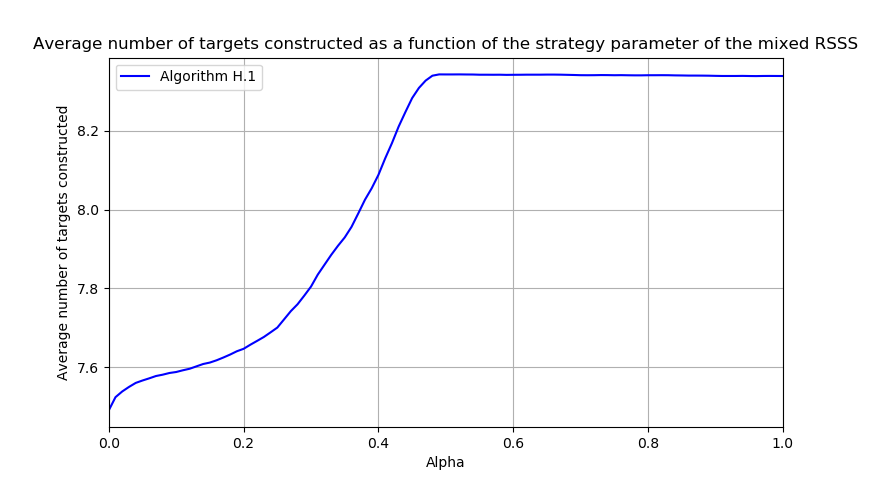
\includegraphics[scale=0.65]{images/locc_counter.png}
    \caption{Average number of succesful target constructions depending on the value of the strategy parameter $\alpha$ for a bank of 9 uniformly sampled states and 1 maximally entangled state, and 10 targets sampled with Dirichlet parameters $\left(2, \frac{1}{2}, \frac{1}{2}, \frac{1}{2}\right)$, sampled over 10000 games. Clearly, the uniqueness entropy is only detrimental for this variant. It has little impact until $\alpha \approx 0.45$, and then the sharp drop seems to indicate that uniqueness entropy becomes significant enough in the loss function under this filtering to kick in and change the selection of states. This can be explained by the fact that more states make it into $Q'_i$ than into $Q''$ (from the original algorithm), and so the value of the uniqueness entropy is generally lower this time.}
    \label{fig:variant_results}
\end{figure}

In Section \ref{sec:strategies_discussion} we showed that improvements over the naive individual strategy are possible using the uniqueness entropy, and perhaps more generally with other lattice-based quantities. However, considering how much of a difference there is between Figures \ref{fig:strategy_comparison} and \ref{fig:variant_results} for such a small change in the filtering process, we hope that other filtering choices could lead to even better improvements over the naive entropic strategy. We were recently made aware of the relevance of the field of dynamic optimization in this context, and hope that it might hold answers to this problem.